%======================================================================
%  Capitulo 4 - Diseno logico de bases de datos
%======================================================================

\section{Diseño lógico de bases de datos}

El diseño lógico transforma el modelo conceptual ajustado del módulo de
operación de envíos (figura~\ref{fig:dmlogico}; en notación de Chen,
figura~\ref{fig:erfinal}) en un modelo relacional:
tablas, columnas, claves primarias y claves foráneas, con sus reglas de
integridad. El resultado tiene 19 tablas, 130 columnas y 27 claves
foráneas.

%-----------------------------------------------------------------------
\subsection{Conversión del diseño conceptual al diseño lógico}

\subsubsection{Modelo Entidad Relación a Modelo Relacional}

La conversión aplica las tres reglas básicas del curso y dos reglas
complementarias para los casos que el modelo del módulo incluye:

\begin{enumerate}[label=\textbf{R\arabic*.},leftmargin=1.2cm,itemsep=2pt]
  \item \textbf{Toda entidad se convierte en tabla}, y su identificador
        en clave primaria. Las 19 entidades dan 19 tablas.
  \item \textbf{Toda relación 1:N se convierte en una propagación de
        clave}: la clave primaria del lado ``uno'' pasa como clave
        foránea a la tabla del lado ``muchos''. Si el mínimo del lado
        ``uno'' es 0, la clave foránea admite nulos.
  \item \textbf{Toda relación N:M se convierte en una tabla intermedia.}
        El módulo no tiene relaciones N:M: la única del prediseño
        (\textit{se asigna}) ya se convirtió en la entidad
        ASIGNACION\_DESPACHO en el ajuste 2.
  \item \textbf{Una relación 1:1 se convierte en una clave foránea única}
        en la tabla de participación opcional (PRUEBA\_ENTREGA y
        NOVEDAD respecto a ASIGNACION\_DESPACHO).
  \item \textbf{Una especialización se convierte en una tabla por
        subtipo}, cuya clave primaria es también clave foránea hacia la
        tabla del supertipo (MENSAJERO respecto a EMPLEADO).
\end{enumerate}

La tabla~\ref{tab:conversion} muestra cómo se convirtió cada relación.

{\singlespacing\small
\begin{longtable}{L{2.0cm} L{1.0cm} L{4.9cm} L{4.6cm} L{1.0cm}}
\caption{Conversión de las relaciones del modelo ER del módulo.}
\label{tab:conversion}\\
\toprule
\textbf{Relación} & \textbf{Regla} & \textbf{Entidades (lado uno -- lado muchos)} & \textbf{Clave foránea resultante} & \textbf{Nulo} \\
\midrule
\endfirsthead
\toprule
\textbf{Relación} & \textbf{Regla} & \textbf{Entidades (lado uno -- lado muchos)} & \textbf{Clave foránea resultante} & \textbf{Nulo} \\
\midrule
\endhead
\bottomrule
\endfoot
\textit{cubre} & R2 & CENTRO\_DISTRIBUCION -- ZONA & zona.id\_centro & No \\
\textit{labora} & R2 & CENTRO\_DISTRIBUCION -- EMPLEADO & empleado.id\_centro & No \\
\textit{dispone} & R2 & CENTRO\_DISTRIBUCION -- VEHICULO & vehiculo.id\_centro & No \\
\textit{origina} & R2 & CENTRO\_DISTRIBUCION -- DESPACHO & despacho.id\_centro & No \\
\textit{ubica} & R2 & ZONA -- SEDE\_CLIENTE & sede\_cliente.id\_zona & No \\
\textit{destina} & R2 & ZONA -- ENVIO & envio.id\_zona & No \\
\textit{atiende} & R2 & ZONA -- MENSAJERO & mensajero.id\_zona & Sí \\
\textit{tiene} & R2 & CLIENTE -- SEDE\_CLIENTE & sede\_cliente.id\_cliente & No \\
\textit{radica} & R2 & CLIENTE -- RECLAMACION & reclamacion.id\_cliente & No \\
\textit{clasifica} & R2 & MODALIDAD -- ENVIO & envio.id\_modalidad & No \\
\textit{solicita} & R2 & SEDE\_CLIENTE -- SOLICITUD\_RECOLECCION & solicitud\_recoleccion.id\_sede & No \\
\textit{contiene} & R2 & SOLICITUD\_RECOLECCION -- ENVIO & envio.id\_solicitud & No \\
\textit{recoge} & R2 & DESPACHO -- SOLICITUD\_RECOLECCION & solicitud\_recoleccion.id\_despacho & Sí \\
\textit{dirigido} & R2 & DESTINATARIO -- ENVIO & envio.id\_destinatario & No \\
\textit{se asigna} & R2 & ENVIO -- ASIGNACION\_DESPACHO & asignacion\_despacho.numero\_guia & No \\
\textit{agrupa} & R2 & DESPACHO -- ASIGNACION\_DESPACHO & asignacion\_despacho.id\_despacho & No \\
\textit{soporta} & R4 & ASIGNACION\_DESPACHO -- PRUEBA\_ENTREGA & prueba\_entrega.id\_asignacion (única) & No \\
\textit{presenta} & R4 & ASIGNACION\_DESPACHO -- NOVEDAD & novedad.id\_asignacion (única) & No \\
\textit{registra} & R2 & ENVIO -- EVENTO\_ENVIO & evento\_envio.numero\_guia & No \\
\textit{indica} & R2 & ESTADO\_ENVIO -- EVENTO\_ENVIO & evento\_envio.id\_estado & No \\
\textit{reporta} & R2 & EMPLEADO -- EVENTO\_ENVIO & evento\_envio.id\_empleado & No \\
\textit{refiere} & R2 & ENVIO -- RECLAMACION & reclamacion.numero\_guia & Sí \\
\textit{usa} & R2 & VEHICULO -- DESPACHO & despacho.id\_vehiculo & No \\
\textit{realiza} & R2 & MENSAJERO -- DESPACHO & despacho.id\_mensajero & No \\
\textit{categoriza} & R2 & TIPO\_VEHICULO -- VEHICULO & vehiculo.id\_tipo\_vehiculo & No \\
\textit{conduce} & R2 & TIPO\_VEHICULO -- MENSAJERO & mensajero.id\_tipo\_vehiculo & No \\
\textit{es un} & R5 & EMPLEADO -- MENSAJERO & mensajero.id\_empleado (PK y FK) & No \\
\end{longtable}
\par}

Las claves foráneas que admiten nulos son exactamente las de las
relaciones con mínimo 0 en el lado ``uno'' (\textit{atiende},
\textit{recoge} y \textit{refiere}); las demás son obligatorias.

\subsubsection{Reglas de Integridad (Propias del Modelo relacional y propias del desarrollador)}

\textbf{Reglas propias del modelo relacional.} Se garantizan con la
estructura de las tablas (tabla~\ref{tab:integridad}).

{\singlespacing\small
\begin{longtable}{L{3.2cm} L{8.2cm} L{2.6cm}}
\caption{Reglas de integridad propias del modelo relacional.}
\label{tab:integridad}\\
\toprule
\textbf{Regla} & \textbf{Cómo se aplica en el módulo} & \textbf{Restricciones} \\
\midrule
\endfirsthead
\toprule
\textbf{Regla} & \textbf{Cómo se aplica en el módulo} & \textbf{Restricciones} \\
\midrule
\endhead
\bottomrule
\endfoot
Integridad de entidad & Cada tabla tiene clave primaria, única y no nula. Se usan claves sustitutas numéricas, salvo ENVIO, cuya clave es el número de guía. Las claves naturales (NIT, documento, placa, nombres de catálogos) se declaran únicas. & 19 PRIMARY KEY, 13 UNIQUE \\
\midrule
Integridad referencial & Toda clave foránea apunta a una fila existente. No se define borrado en cascada: la política de acceso prohíbe eliminar registros, que se anulan por estado, así que el motor rechaza borrar una fila referenciada. & 27 FOREIGN KEY \\
\midrule
Integridad de dominio & Cada columna tiene tipo y tamaño; las obligatorias son NOT NULL; los estados y tipos solo admiten los valores de su lista, y los estados iniciales tienen valor por defecto. & 110 NOT NULL, 33 CHECK, 12 DEFAULT \\
\end{longtable}
\par}

\textbf{Reglas propias del desarrollador.} Son las reglas de negocio
que salen de las políticas y de la caracterización de los procesos
(tabla~\ref{tab:reglasnegocio}). Las que se pueden expresar sobre una
sola fila o con unicidad ya están en el modelo lógico; las que
dependen de otras filas o tablas se implementarán con disparadores,
procedimientos y permisos en el diseño físico.

{\singlespacing\small
\begin{longtable}{L{1.0cm} L{6.6cm} L{2.6cm} L{4.2cm}}
\caption{Reglas de negocio del módulo.}
\label{tab:reglasnegocio}\\
\toprule
\textbf{Cód.} & \textbf{Regla} & \textbf{Origen} & \textbf{Implementación} \\
\midrule
\endfirsthead
\toprule
\textbf{Cód.} & \textbf{Regla} & \textbf{Origen} & \textbf{Implementación} \\
\midrule
\endhead
\bottomrule
\endfoot
RN01 & Cada envío tiene un número de guía único. & Calidad del servicio & PK de envio \\
RN02 & Todo envío se registra con destinatario, dirección, zona, modalidad, peso, contenido y fecha de compromiso. & Calidad del servicio & NOT NULL en envio \\
RN03 & La fecha de compromiso no es anterior a la de registro, los pesos y el flete son positivos y el valor declarado no es negativo. & P1 & CHECK envio\_compromiso\_ck, envio\_pesos\_ck, envio\_valor\_ck \\
RN04 & Un destinatario existe una sola vez (tipo y número de documento). & Datos personales & UNIQUE destinatario\_documento\_uk \\
RN05 & Ningún envío se marca como entregado sin prueba de entrega. & Calidad del servicio & Disparador (diseño físico) \\
RN06 & Los envíos frágiles o de alto valor solo se entregan al destinatario: el documento de quien recibe debe ser el del destinatario. & Manejo de la mercancía & Disparador (diseño físico) \\
RN07 & Máximo dos intentos de entrega; el tercero solo puede ser la devolución y solo después de dos novedades. & P3 & CHECK asignacion\_intento\_ck, UNIQUE asignacion\_intento\_uk y disparador \\
RN08 & Cada intento tiene como máximo una prueba de entrega o una novedad. & P2 & UNIQUE prueba\_asignacion\_uk, novedad\_asignacion\_uk \\
RN09 & Solo un mensajero puede realizar un despacho. & Seguridad vial & FK despacho\_mensajero\_fk \\
RN10 & Al crear un despacho, el vehículo debe estar DISPONIBLE y el mensajero ACTIVO (la validación de documentos, licencia y capacitación se agrega con M3 y M4). & Seguridad vial & Disparador (diseño físico) \\
RN11 & El vehículo del despacho debe ser del tipo que conduce el mensajero. & Seguridad vial & Disparador (diseño físico) \\
RN12 & Todo envío nace con el evento REGISTRADO y sus estados siguen el ciclo de vida (no se pasa a ENTREGADO sin haber estado EN\_RUTA). & Seguimiento por eventos & Procedimiento de registro y disparador \\
RN13 & Cada evento registra el empleado responsable. & Manejo de la mercancía & FK NOT NULL evento\_empleado\_fk \\
RN14 & La respuesta a una reclamación es posterior a su radicación; la meta de cuatro horas se mide como indicador. & OE2 & CHECK reclamacion\_resp\_ck y vista \\
RN15 & Solo se registran solicitudes de clientes activos (hasta integrar los contratos de M2). & P1 & Disparador (diseño físico) \\
RN16 & No se eliminan registros; se anulan o cierran por estado. & Acceso a la información & Permisos sin DELETE (diseño físico) \\
\end{longtable}
\par}

\subsubsection{Optimización del Diseño Lógico de la BD}

Antes de normalizar se tomaron las siguientes decisiones de diseño:

\begin{enumerate}[label=\arabic*.,leftmargin=1.2cm,itemsep=2pt]
  \item \textbf{Claves.} El número de guía es la clave de ENVIO porque
        es estable, va impreso en el paquete y es lo que el cliente
        consulta. Las demás tablas usan claves sustitutas numéricas, más
        cortas y estables que las naturales, que se conservan como
        únicas.
  \item \textbf{Estado actual del envío.} No se guarda en ENVIO, porque
        se deduce del último evento y guardarlo dos veces permitiría
        contradicciones (ajuste 4). Se obtiene con la vista
        v\_estado\_actual\_envio; si en el diseño físico se necesita por
        rendimiento, se agregará como dato derivado mantenido por un
        disparador.
  \item \textbf{Prueba y novedad en tablas propias.} Podrían ser columnas
        de ASIGNACION\_DESPACHO, pero cada intento tiene una u otra, nunca
        las dos, y la mayoría de columnas quedaría nula. Separarlas con
        una clave foránea única evita los nulos y permite reglas propias
        para cada una.
  \item \textbf{Mensajero como tabla de subtipo.} Guardar la zona y el
        tipo de vehículo en EMPLEADO dejaría esas columnas vacías para
        quien no es mensajero, y no impediría asignar un despacho a otro
        cargo. La tabla MENSAJERO resuelve ambas cosas.
  \item \textbf{Catálogos frente a listas fijas.} Son tablas los
        dominios que tienen atributos propios o que usan las reglas
        (estados del envío, modalidades, tipos de vehículo); son listas
        CHECK los dominios simples que no cambian (franja horaria, tipo
        de prueba, tipo de novedad).
  \item \textbf{Resultado del intento.} El dominio de
        asignacion\_despacho.resultado queda en PENDIENTE, ENTREGADO,
        NOVEDAD y DEVUELTO, y el número de intento entre 1 y 3: los dos
        primeros son de entrega y el tercero es la devolución.
  \item \textbf{Integración futura.} Las columnas que dependen de otros
        módulos (envio.id\_factura, reclamacion.id\_factura) no se crean
        todavía; al integrar M2 se agregan sin modificar las columnas
        existentes.
\end{enumerate}

\subsubsection{Normalización y Formas Normales}

La normalización detecta y elimina redundancias que causan anomalías de
inserción, actualización y borrado. Una tabla está en primera forma
normal (1FN) si todos sus valores son atómicos; en segunda (2FN) si
está en 1FN y cada atributo no clave depende de la clave completa; en
tercera (3FN) si está en 2FN y ningún atributo no clave depende de otro
atributo no clave; y en forma normal de Boyce-Codd (FNBC) si todo
determinante es clave candidata.

Para comprobar el diseño se parte de cómo vería los datos alguien que
no ha modelado: una sola tabla con todo lo que se anota de una guía.

\begin{sloppypar}\noindent\textbf{Forma no normalizada.} GUIA(\pk{numero\_guia}, fecha\_registro,
nit\_cliente, razon\_social, direccion\_sede, zona\_sede,
documento\_destinatario, nombre\_destinatario, telefono\_destinatario,
direccion\_destino, zona\_destino, centro\_zona, modalidad,
plazo\_modalidad, peso\_declarado, peso\_real, contenido,
valor\_declarado, fragil, alto\_valor, valor\_flete, fecha\_compromiso,
\{fecha\_hora\_evento, estado, documento\_empleado, nombre\_empleado\},
\{id\_despacho, fecha\_despacho, placa, tipo\_vehiculo, capacidad\_tipo,
documento\_mensajero, nombre\_mensajero, orden\_visita, intento,
resultado, quien\_recibe, tipo\_prueba, tipo\_novedad,
descripcion\_novedad\}). Las llaves marcan grupos repetitivos: una guía
tiene varios eventos y varias visitas.\end{sloppypar}

\begin{sloppypar}\noindent\textbf{Primera forma normal.} Los grupos repetitivos salen a tablas
propias con la clave de la guía:
EVENTO(\pk{numero\_guia, fecha\_hora}, estado, documento\_empleado,
nombre\_empleado) y VISITA(\pk{numero\_guia, id\_despacho},
fecha\_despacho, placa, tipo\_vehiculo, capacidad\_tipo,
documento\_mensajero, nombre\_mensajero, orden\_visita, intento,
resultado, quien\_recibe, tipo\_prueba, tipo\_novedad,
descripcion\_novedad).\end{sloppypar}

\begin{sloppypar}\noindent\textbf{Segunda forma normal.} En VISITA, fecha\_despacho, placa,
tipo\_vehiculo, capacidad\_tipo y los datos del mensajero dependen solo
de id\_despacho, que es parte de la clave. Se separan en
DESPACHO(\pk{id\_despacho}, fecha, placa, tipo\_vehiculo,
capacidad\_tipo, documento\_mensajero, nombre\_mensajero). GUIA y
EVENTO ya cumplen 2FN: GUIA tiene clave simple y en EVENTO todos los
atributos dependen de la guía y del momento juntos.\end{sloppypar}

\textbf{Tercera forma normal.} Se eliminan las dependencias
transitivas:

\begin{itemize}[leftmargin=1.2cm,itemsep=1pt]
  \item En GUIA: documento\_destinatario $\rightarrow$ nombre, teléfono
        (sale DESTINATARIO); la guía pertenece a una solicitud, la
        solicitud a una sede y la sede a un cliente: sede $\rightarrow$
        cliente, dirección, zona y nit $\rightarrow$ razón social (salen
        SOLICITUD\_RECOLECCION, SEDE\_CLIENTE y CLIENTE); zona
        $\rightarrow$ centro (salen ZONA y CENTRO\_DISTRIBUCION);
        modalidad $\rightarrow$ plazo (sale MODALIDAD).
  \item En EVENTO: documento\_empleado $\rightarrow$ nombre (sale
        EMPLEADO) y estado $\rightarrow$ es\_final (sale ESTADO\_ENVIO).
  \item En DESPACHO: placa $\rightarrow$ tipo, marca, capacidad y tipo
        $\rightarrow$ capacidad máxima (salen VEHICULO y TIPO\_VEHICULO);
        documento\_mensajero $\rightarrow$ nombre (sale MENSAJERO, con
        sus datos de empleado en EMPLEADO).
  \item En VISITA no hay dependencias transitivas, pero los datos de
        prueba y de novedad son excluyentes y casi siempre nulos; por la
        decisión 3 de optimización salen a PRUEBA\_ENTREGA y NOVEDAD, y
        VISITA toma el nombre ASIGNACION\_DESPACHO con una clave
        sustituta.
\end{itemize}

\textbf{Forma normal de Boyce-Codd.} En las tablas resultantes todo
determinante es clave candidata (tabla~\ref{tab:formasnormales}). Las
únicas tablas con más de una clave candidata son DESTINATARIO, cuyo
documento también la identifica, y ASIGNACION\_DESPACHO, que también se
identifica por (guía, despacho) y por (guía, intento); ambas se declaran
únicas. El resultado coincide con las tablas obtenidas por conversión
del modelo ER, lo que confirma que el diseño conceptual era correcto.

{\singlespacing\small
\begin{longtable}{L{3.6cm} L{3.8cm} L{5.4cm} L{1.2cm}}
\caption{Dependencias funcionales y forma normal de cada tabla.}
\label{tab:formasnormales}\\
\toprule
\textbf{Tabla} & \textbf{Claves candidatas} & \textbf{Dependencias funcionales} & \textbf{FN} \\
\midrule
\endfirsthead
\toprule
\textbf{Tabla} & \textbf{Claves candidatas} & \textbf{Dependencias funcionales} & \textbf{FN} \\
\midrule
\endhead
\bottomrule
\endfoot
centro\_distribucion & id\_centro; nombre & id\_centro $\rightarrow$ resto; nombre $\rightarrow$ id\_centro & FNBC \\
zona & id\_zona; nombre & id\_zona $\rightarrow$ resto; nombre $\rightarrow$ id\_zona & FNBC \\
cliente & id\_cliente; nit & id\_cliente $\rightarrow$ resto; nit $\rightarrow$ id\_cliente & FNBC \\
sede\_cliente & id\_sede & id\_sede $\rightarrow$ resto & FNBC \\
modalidad & id\_modalidad; nombre & id\_modalidad $\rightarrow$ resto; nombre $\rightarrow$ id\_modalidad & FNBC \\
tipo\_vehiculo & id\_tipo\_vehiculo; nombre & id\_tipo\_vehiculo $\rightarrow$ resto; nombre $\rightarrow$ id\_tipo\_vehiculo & FNBC \\
vehiculo & id\_vehiculo; placa (si existe) & id\_vehiculo $\rightarrow$ resto; placa $\rightarrow$ id\_vehiculo & FNBC \\
empleado & id\_empleado; documento & id\_empleado $\rightarrow$ resto; documento $\rightarrow$ id\_empleado & FNBC \\
mensajero & id\_empleado & id\_empleado $\rightarrow$ id\_zona, id\_tipo\_vehiculo & FNBC \\
destinatario & id\_destinatario; (tipo\_documento, numero\_documento) & id\_destinatario $\rightarrow$ resto; documento $\rightarrow$ id\_destinatario & FNBC \\
despacho & id\_despacho & id\_despacho $\rightarrow$ resto & FNBC \\
solicitud\_recoleccion & id\_solicitud & id\_solicitud $\rightarrow$ resto & FNBC \\
envio & numero\_guia & numero\_guia $\rightarrow$ resto & FNBC \\
asignacion\_despacho & id\_asignacion; (numero\_guia, id\_despacho); (numero\_guia, numero\_intento) & cada clave $\rightarrow$ resto & FNBC \\
estado\_envio & id\_estado; nombre & id\_estado $\rightarrow$ resto; nombre $\rightarrow$ id\_estado & FNBC \\
evento\_envio & id\_evento & id\_evento $\rightarrow$ resto & FNBC \\
prueba\_entrega & id\_prueba; id\_asignacion & cada clave $\rightarrow$ resto & FNBC \\
novedad & id\_novedad; id\_asignacion & cada clave $\rightarrow$ resto & FNBC \\
reclamacion & id\_reclamacion & id\_reclamacion $\rightarrow$ resto & FNBC \\
\end{longtable}
\par}

\subsubsection{Diseño Lógico de la Base de Datos -- Modelo Relacional}
\label{sec:esquemarel}

La figura~\ref{fig:dmrelacional} presenta el modelo relacional del
módulo, construido en Data Modeler. En cada tabla,
\texttt{P} marca la clave primaria, \texttt{F} una clave foránea,
\texttt{U} un valor único y \texttt{*} una columna obligatoria; cada
línea entre tablas es una clave foránea. Tiene 19 tablas con sus 19 claves
primarias, las 13 restricciones de unicidad, las 27 claves foráneas con
sus nombres. Las vistas de usuario no se dibujan en el diagrama, porque no
tienen claves foráneas; se describen más adelante. Una versión elaborada en draw.io, que indica
junto a cada clave foránea la tabla a la que apunta, está en la
figura~\ref{fig:relacional} del anexo~\ref{anx:chen}.


En notación de esquema relacional (clave primaria subrayada, claves
foráneas en cursiva):

{\singlespacing\small\sloppy
\begin{itemize}[leftmargin=0.6cm,itemsep=3pt,label={}]
  \item \textbf{CENTRO\_DISTRIBUCION}(\pk{id\_centro}, nombre, direccion, telefono, estado)
  \item \textbf{ZONA}(\pk{id\_zona}, \fk{id\_centro}, nombre, localidades)
  \item \textbf{CLIENTE}(\pk{id\_cliente}, nit, razon\_social, tipo\_cliente, telefono, correo, fecha\_vinculacion, estado)
  \item \textbf{SEDE\_CLIENTE}(\pk{id\_sede}, \fk{id\_cliente}, \fk{id\_zona}, nombre, direccion, contacto, telefono)
  \item \textbf{MODALIDAD}(\pk{id\_modalidad}, nombre, plazo\_dias\_habiles)
  \item \textbf{TIPO\_VEHICULO}(\pk{id\_tipo\_vehiculo}, nombre, capacidad\_max\_kg)
  \item \textbf{VEHICULO}(\pk{id\_vehiculo}, \fk{id\_centro}, \fk{id\_tipo\_vehiculo}, placa, marca, modelo, capacidad\_kg, electrico, estado)
  \item \textbf{EMPLEADO}(\pk{id\_empleado}, \fk{id\_centro}, documento, nombres, apellidos, cargo, telefono, correo, fecha\_ingreso, fecha\_retiro, motivo\_retiro, estado)
  \item \textbf{MENSAJERO}(\pk{\fk{id\_empleado}}, \fk{id\_zona}, \fk{id\_tipo\_vehiculo})
  \item \textbf{DESTINATARIO}(\pk{id\_destinatario}, tipo\_documento, numero\_documento, nombre, telefono, correo)
  \item \textbf{DESPACHO}(\pk{id\_despacho}, \fk{id\_centro}, \fk{id\_vehiculo}, \fk{id\_mensajero}, fecha, tipo, hora\_salida, hora\_cierre, estado)
  \item \textbf{SOLICITUD\_RECOLECCION}(\pk{id\_solicitud}, \fk{id\_sede}, \fk{id\_despacho}, fecha\_solicitud, fecha\_programada, franja\_horaria, estado)
  \item \textbf{ENVIO}(\pk{numero\_guia}, \fk{id\_solicitud}, \fk{id\_destinatario}, \fk{id\_zona}, \fk{id\_modalidad}, fecha\_registro, direccion\_destino, peso\_declarado, peso\_real, contenido, valor\_declarado, fragil, alto\_valor, valor\_flete, fecha\_compromiso)
  \item \textbf{ASIGNACION\_DESPACHO}(\pk{id\_asignacion}, \fk{numero\_guia}, \fk{id\_despacho}, numero\_intento, orden\_visita, hora\_visita, resultado)
  \item \textbf{ESTADO\_ENVIO}(\pk{id\_estado}, nombre, es\_final)
  \item \textbf{EVENTO\_ENVIO}(\pk{id\_evento}, \fk{numero\_guia}, \fk{id\_estado}, \fk{id\_empleado}, fecha\_hora, observacion)
  \item \textbf{PRUEBA\_ENTREGA}(\pk{id\_prueba}, \fk{id\_asignacion}, fecha\_hora, nombre\_receptor, documento\_receptor, tipo\_prueba, archivo\_soporte)
  \item \textbf{NOVEDAD}(\pk{id\_novedad}, \fk{id\_asignacion}, tipo\_novedad, descripcion, accion, solucion, estado)
  \item \textbf{RECLAMACION}(\pk{id\_reclamacion}, \fk{id\_cliente}, \fk{numero\_guia}, fecha\_radicacion, tipo, descripcion, respuesta, fecha\_respuesta, estado)
\end{itemize}
\par}
\begin{landscape}
{\singlespacing
\begin{figure}[p]
\centering
\adjustbox{max width=22.5cm, max totalheight=14.6cm}{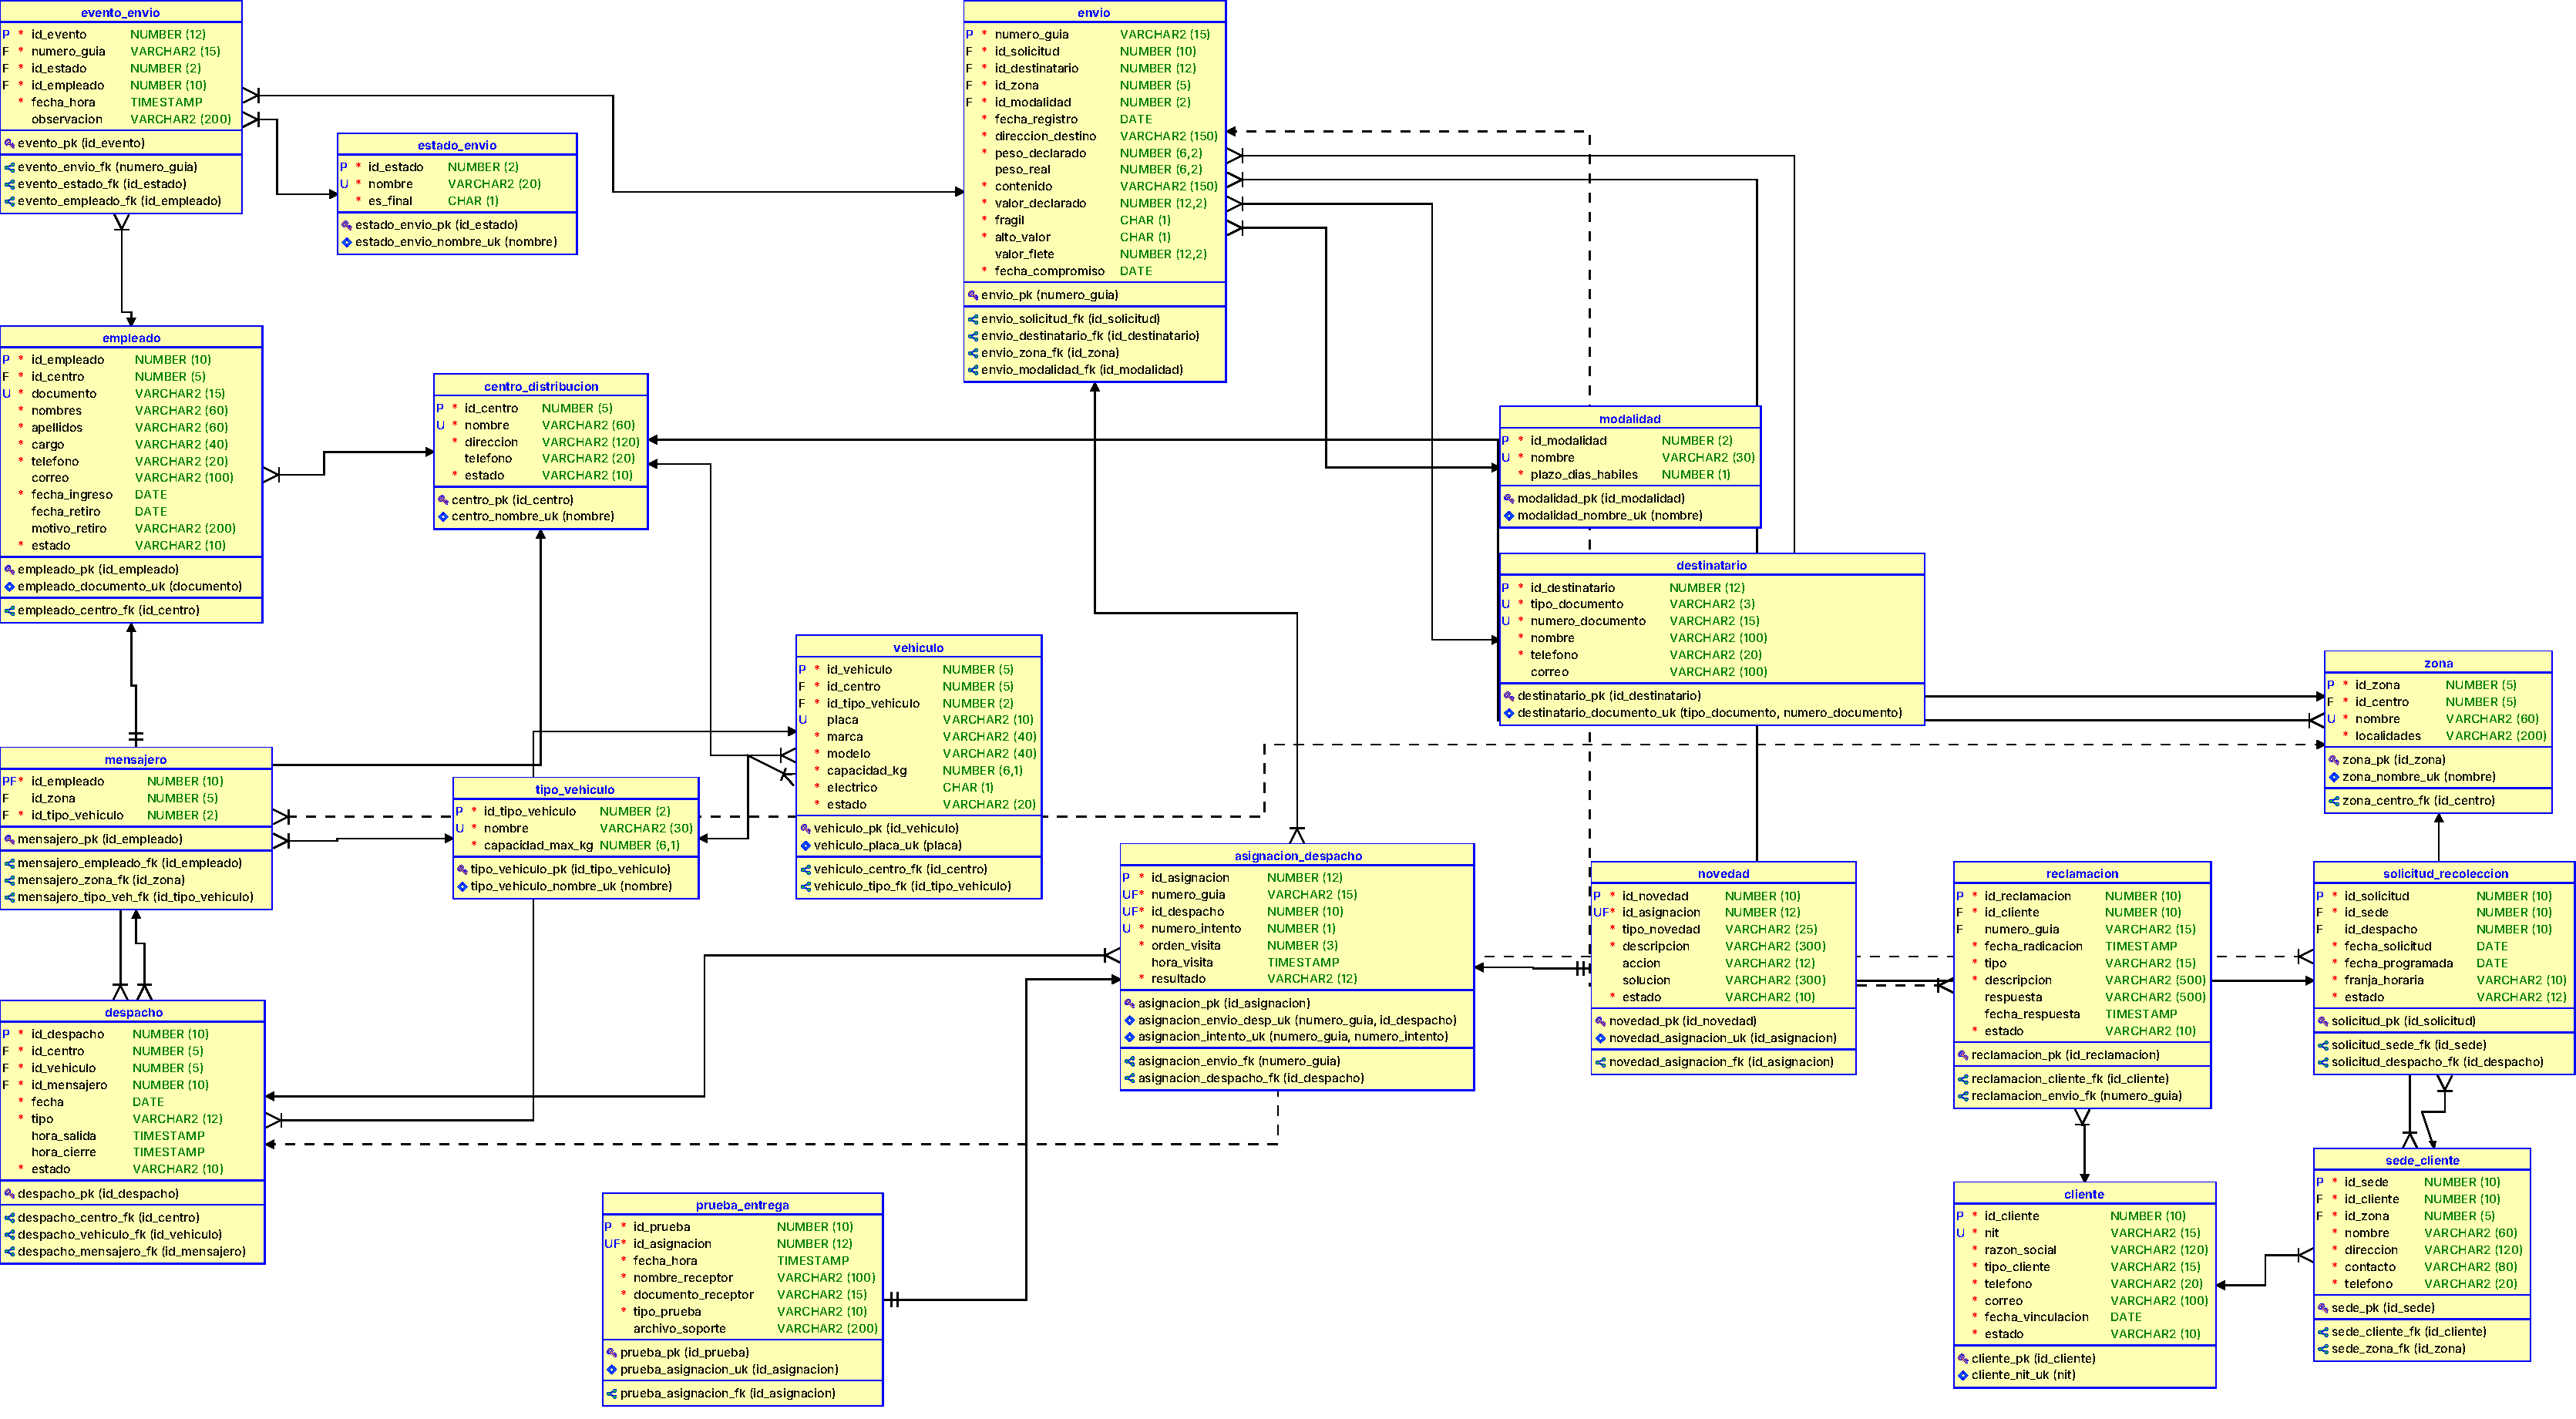
\includegraphics{figuras/datamodeler/dm_M_relacional.pdf}}
\caption{Modelo relacional del módulo en Data Modeler.}
\label{fig:dmrelacional}
\end{figure}
\par}
\end{landscape}

\paragraph{Vistas de usuario (esquema externo)}

Cada usuario del módulo accede a los datos mediante vistas que reúnen lo
que necesita sin exponerle el resto (tabla~\ref{tab:vistas}). Las vistas
también implementan el estado actual del envío (decisión 2 de
optimización) y los indicadores de operación. Por ejemplo, la vista
del estado actual reúne cada envío con su cliente, su zona y su
modalidad, y toma como estado el de su evento más reciente.

{\singlespacing\small
\begin{longtable}{L{3.6cm} L{1.4cm} L{5.6cm} L{3.8cm}}
\caption{Vistas de usuario del módulo (esquema externo).}
\label{tab:vistas}\\
\toprule
\textbf{Vista} & \textbf{Usu.} & \textbf{Propósito} & \textbf{Tablas base} \\
\midrule
\endfirsthead
\toprule
\textbf{Vista} & \textbf{Usu.} & \textbf{Propósito} & \textbf{Tablas base} \\
\midrule
\endhead
\bottomrule
\endfoot
v\_seguimiento\_envio & U3, U9 & Recorrido completo de un envío por número de guía. El cliente (U9) la consulta filtrada por su id\_cliente. & envio, solicitud\_recoleccion, sede\_cliente, evento\_envio, estado\_envio, empleado \\
\midrule
v\_estado\_actual\_envio & U1, U2, U3 & Estado actual de cada envío (el de su último evento), con cliente, zona, modalidad y fecha de compromiso. & envio, solicitud\_recoleccion, sede\_cliente, cliente, zona, modalidad, evento\_envio, estado\_envio \\
\midrule
v\_planilla\_despacho & U2, U4 & Planilla de ruta: envíos de cada despacho en orden de visita, con datos del destinatario y del mensajero. & despacho, asignacion\_despacho, envio, destinatario, zona, vehiculo, empleado \\
\midrule
v\_envios\_por\_despachar & U2 & Envíos clasificados que todavía no están en un despacho de entrega abierto, por zona y modalidad, para armar las rutas. & v\_estado\_actual\_envio, envio, asignacion\_despacho, despacho \\
\midrule
v\_novedades\_abiertas & U3 & Novedades sin cerrar, con el intento en que ocurrieron y los datos para contactar al destinatario y al cliente. & novedad, asignacion\_despacho, envio, destinatario, solicitud\_recoleccion, sede\_cliente, cliente \\
\midrule
v\_reclamaciones\_pendientes & U1, U3 & Reclamaciones abiertas, con el cliente y el envío reclamado; insumo del indicador de tiempo de respuesta. & reclamacion, cliente \\
\midrule
v\_cumplimiento\_entregas & U1 & Por centro y zona: envíos entregados y cuántos se entregaron dentro de la fecha de compromiso (indicador de OE1). & envio, zona, evento\_envio, estado\_envio \\
\end{longtable}
\par}

\subsubsection{Documentación de la BD -- Diccionario de Datos}
\label{sec:diccionario}

El diccionario de datos (tabla~\ref{tab:diccionario}) describe cada
columna del módulo: tipo de dato de Oracle, si admite nulos, su papel en
las claves y su significado. Las listas de valores permitidos y los
valores por defecto corresponden a las restricciones de dominio de la
tabla~\ref{tab:integridad}. Los estados del envío del catálogo ESTADO\_ENVIO son
REGISTRADO, RECOLECTADO, EN\_CENTRO, CLASIFICADO, EN\_RUTA, ENTREGADO,
CON\_NOVEDAD, DEVUELTO y ANULADO.
Las descripciones también se registraron en Data Modeler, en el campo
\textit{Comment in RDBMS} de cada tabla y columna. El reporte de tablas
generado por la herramienta y su comparación con este diccionario están
en el anexo~\ref{anx:dmdiccionario}.

{\singlespacing\footnotesize
\begin{longtable}{L{3.3cm} L{2.6cm} L{0.8cm} L{1.2cm} L{5.8cm}}
\caption{Diccionario de datos del módulo de operación de envíos.}
\label{tab:diccionario}\\
\toprule
\textbf{Columna} & \textbf{Tipo} & \textbf{Nulo} & \textbf{Clave} & \textbf{Descripción} \\
\midrule
\endfirsthead
\toprule
\textbf{Columna} & \textbf{Tipo} & \textbf{Nulo} & \textbf{Clave} & \textbf{Descripción} \\
\midrule
\endhead
\bottomrule
\endfoot
\multicolumn{5}{L{15.4cm}}{\textbf{centro\_distribucion} -- Centro donde se reciben, clasifican y despachan los envíos. \textit{(Estructura operativa)}} \\*
\midrule
id\_centro & NUMBER(5) & No & PK & Identificador del centro \\
nombre & VARCHAR2(60) & No & UK & Nombre del centro \\
direccion & VARCHAR2(120) & No &  & Dirección \\
telefono & VARCHAR2(20) & Sí &  & Teléfono de contacto \\
estado & VARCHAR2(10) & No &  & ACTIVO o INACTIVO; por defecto ACTIVO \\
\midrule
\multicolumn{5}{L{15.4cm}}{\textbf{zona} -- Sector de la ciudad atendido por un centro. \textit{(Estructura operativa)}} \\*
\midrule
id\_zona & NUMBER(5) & No & PK & Identificador de la zona \\
id\_centro & NUMBER(5) & No & FK & Centro que atiende la zona (ref. centro\_distribucion) \\
nombre & VARCHAR2(60) & No & UK & Nombre de la zona \\
localidades & VARCHAR2(200) & No &  & Localidades que cubre \\
\midrule
\multicolumn{5}{L{15.4cm}}{\textbf{cliente} -- Empresa que contrata el servicio. \textit{(Referencia (comercial))}} \\*
\midrule
id\_cliente & NUMBER(10) & No & PK & Identificador del cliente \\
nit & VARCHAR2(15) & No & UK & NIT \\
razon\_social & VARCHAR2(120) & No &  & Razón social \\
tipo\_cliente & VARCHAR2(15) & No &  & TIENDA\_LINEA, DROGUERIA u OFICINA \\
telefono & VARCHAR2(20) & No &  & Teléfono \\
correo & VARCHAR2(100) & No &  & Correo electrónico \\
fecha\_vinculacion & DATE & No &  & Fecha de vinculación \\
estado & VARCHAR2(10) & No &  & ACTIVO o INACTIVO; por defecto ACTIVO \\
\midrule
\multicolumn{5}{L{15.4cm}}{\textbf{sede\_cliente} -- Punto de recolección de un cliente. \textit{(Referencia (comercial))}} \\*
\midrule
id\_sede & NUMBER(10) & No & PK & Identificador de la sede \\
id\_cliente & NUMBER(10) & No & FK & Cliente dueño de la sede (ref. cliente) \\
id\_zona & NUMBER(5) & No & FK & Zona donde está la sede (ref. zona) \\
nombre & VARCHAR2(60) & No &  & Nombre de la sede \\
direccion & VARCHAR2(120) & No &  & Dirección \\
contacto & VARCHAR2(80) & No &  & Persona de contacto \\
telefono & VARCHAR2(20) & No &  & Teléfono \\
\midrule
\multicolumn{5}{L{15.4cm}}{\textbf{modalidad} -- Tipo de servicio según el tiempo de entrega. \textit{(Referencia (comercial))}} \\*
\midrule
id\_modalidad & NUMBER(2) & No & PK & Identificador \\
nombre & VARCHAR2(30) & No & UK & MISMO\_DIA, DIA\_SIGUIENTE o ESTANDAR \\
plazo\_dias\_habiles & NUMBER(1) & No &  & Plazo de entrega en días hábiles \\
\midrule
\multicolumn{5}{L{15.4cm}}{\textbf{tipo\_vehiculo} -- Catálogo de tipos de vehículo. \textit{(Referencia (flota))}} \\*
\midrule
id\_tipo\_vehiculo & NUMBER(2) & No & PK & Identificador \\
nombre & VARCHAR2(30) & No & UK & MOTOCICLETA, FURGONETA o BICICLETA\_ELECTRICA \\
capacidad\_max\_kg & NUMBER(6,1) & No &  & Carga máxima del tipo \\
\midrule
\multicolumn{5}{L{15.4cm}}{\textbf{vehiculo} -- Vehículo de la flota. \textit{(Referencia (flota))}} \\*
\midrule
id\_vehiculo & NUMBER(5) & No & PK & Identificador \\
id\_centro & NUMBER(5) & No & FK & Centro al que está asignado (ref. centro\_distribucion) \\
id\_tipo\_vehiculo & NUMBER(2) & No & FK & Tipo de vehículo (ref. tipo\_vehiculo) \\
placa & VARCHAR2(10) & Sí & UK & Placa (nula en bicicletas) \\
marca & VARCHAR2(40) & No &  & Marca \\
modelo & VARCHAR2(40) & No &  & Modelo \\
capacidad\_kg & NUMBER(6,1) & No &  & Carga máxima del vehículo \\
electrico & CHAR(1) & No &  & S o N \\
estado & VARCHAR2(20) & No &  & DISPONIBLE, EN\_MANTENIMIENTO o FUERA\_SERVICIO; por defecto DISPONIBLE \\
\midrule
\multicolumn{5}{L{15.4cm}}{\textbf{empleado} -- Persona vinculada a la empresa. \textit{(Referencia (talento humano))}} \\*
\midrule
id\_empleado & NUMBER(10) & No & PK & Identificador \\
id\_centro & NUMBER(5) & No & FK & Centro donde labora (ref. centro\_distribucion) \\
documento & VARCHAR2(15) & No & UK & Documento de identidad \\
nombres & VARCHAR2(60) & No &  & Nombres \\
apellidos & VARCHAR2(60) & No &  & Apellidos \\
cargo & VARCHAR2(40) & No &  & Cargo \\
telefono & VARCHAR2(20) & No &  & Teléfono \\
correo & VARCHAR2(100) & Sí &  & Correo electrónico \\
fecha\_ingreso & DATE & No &  & Fecha de ingreso \\
fecha\_retiro & DATE & Sí &  & Fecha de retiro \\
motivo\_retiro & VARCHAR2(200) & Sí &  & Motivo del retiro \\
estado & VARCHAR2(10) & No &  & ACTIVO o RETIRADO; por defecto ACTIVO \\
\midrule
\multicolumn{5}{L{15.4cm}}{\textbf{mensajero} -- Empleado que sale a ruta (subtipo de EMPLEADO). \textit{(Referencia (talento humano))}} \\*
\midrule
id\_empleado & NUMBER(10) & No & PK, FK & Mismo identificador del empleado (ref. empleado) \\
id\_zona & NUMBER(5) & Sí & FK & Zona fija asignada (opcional) (ref. zona) \\
id\_tipo\_vehiculo & NUMBER(2) & No & FK & Tipo de vehículo que conduce (ref. tipo\_vehiculo) \\
\midrule
\multicolumn{5}{L{15.4cm}}{\textbf{destinatario} -- Persona que recibe los envíos. \textit{(Operación de envíos)}} \\*
\midrule
id\_destinatario & NUMBER(12) & No & PK & Identificador \\
tipo\_documento & VARCHAR2(3) & No & UK & CC, CE, NIT, PAS o TI \\
numero\_documento & VARCHAR2(15) & No & UK & Número de documento \\
nombre & VARCHAR2(100) & No &  & Nombre completo \\
telefono & VARCHAR2(20) & No &  & Teléfono \\
correo & VARCHAR2(100) & Sí &  & Correo electrónico \\
\midrule
\multicolumn{5}{L{15.4cm}}{\textbf{despacho} -- Salida de un mensajero con un vehículo. \textit{(Operación de envíos)}} \\*
\midrule
id\_despacho & NUMBER(10) & No & PK & Identificador \\
id\_centro & NUMBER(5) & No & FK & Centro de origen (ref. centro\_distribucion) \\
id\_vehiculo & NUMBER(5) & No & FK & Vehículo asignado (ref. vehiculo) \\
id\_mensajero & NUMBER(10) & No & FK & Mensajero asignado (ref. mensajero) \\
fecha & DATE & No &  & Fecha del despacho \\
tipo & VARCHAR2(12) & No &  & RECOLECCION o ENTREGA \\
hora\_salida & TIMESTAMP & Sí &  & Hora de salida \\
hora\_cierre & TIMESTAMP & Sí &  & Hora de cierre de la ruta \\
estado & VARCHAR2(10) & No &  & ARMADO, EN\_RUTA o CERRADO; por defecto ARMADO \\
\midrule
\multicolumn{5}{L{15.4cm}}{\textbf{solicitud\_recoleccion} -- Pedido de recolección en una sede del cliente. \textit{(Operación de envíos)}} \\*
\midrule
id\_solicitud & NUMBER(10) & No & PK & Identificador \\
id\_sede & NUMBER(10) & No & FK & Sede donde se recoge (ref. sede\_cliente) \\
id\_despacho & NUMBER(10) & Sí & FK & Despacho de recolección (al programarla) (ref. despacho) \\
fecha\_solicitud & DATE & No &  & Fecha en que se pide \\
fecha\_programada & DATE & No &  & Fecha de recolección \\
franja\_horaria & VARCHAR2(10) & No &  & MANANA o TARDE \\
estado & VARCHAR2(12) & No &  & PENDIENTE, PROGRAMADA, ATENDIDA o NO\_ATENDIDA; por defecto PENDIENTE \\
\midrule
\multicolumn{5}{L{15.4cm}}{\textbf{envio} -- Paquete o documento identificado por su guía. \textit{(Operación de envíos)}} \\*
\midrule
numero\_guia & VARCHAR2(15) & No & PK & Número de guía \\
id\_solicitud & NUMBER(10) & No & FK & Solicitud en la que se recoge (ref. solicitud\_recoleccion) \\
id\_destinatario & NUMBER(12) & No & FK & Destinatario (ref. destinatario) \\
id\_zona & NUMBER(5) & No & FK & Zona de destino (ref. zona) \\
id\_modalidad & NUMBER(2) & No & FK & Modalidad contratada (ref. modalidad) \\
fecha\_registro & DATE & No &  & Fecha de registro \\
direccion\_destino & VARCHAR2(150) & No &  & Dirección de entrega \\
peso\_declarado & NUMBER(6,2) & No &  & Peso declarado en kg \\
peso\_real & NUMBER(6,2) & Sí &  & Peso verificado en el centro \\
contenido & VARCHAR2(150) & No &  & Descripción del contenido \\
valor\_declarado & NUMBER(12,2) & No &  & Valor declarado \\
fragil & CHAR(1) & No &  & S o N; por defecto N \\
alto\_valor & CHAR(1) & No &  & S o N; por defecto N \\
valor\_flete & NUMBER(12,2) & Sí &  & Valor cobrado por el envío \\
fecha\_compromiso & DATE & No &  & Fecha máxima de entrega \\
\midrule
\multicolumn{5}{L{15.4cm}}{\textbf{asignacion\_despacho} -- Cada intento de un envío en un despacho. \textit{(Operación de envíos)}} \\*
\midrule
id\_asignacion & NUMBER(12) & No & PK & Identificador \\
numero\_guia & VARCHAR2(15) & No & FK, UK & Envío (ref. envio) \\
id\_despacho & NUMBER(10) & No & FK, UK & Despacho (ref. despacho) \\
numero\_intento & NUMBER(1) & No & UK & 1 y 2: entrega; 3: devolución \\
orden\_visita & NUMBER(3) & No &  & Orden de visita en la ruta \\
hora\_visita & TIMESTAMP & Sí &  & Hora en que se visitó \\
resultado & VARCHAR2(12) & No &  & PENDIENTE, ENTREGADO, NOVEDAD o DEVUELTO; por defecto PENDIENTE \\
\midrule
\multicolumn{5}{L{15.4cm}}{\textbf{estado\_envio} -- Catálogo de estados del envío. \textit{(Operación de envíos)}} \\*
\midrule
id\_estado & NUMBER(2) & No & PK & Identificador \\
nombre & VARCHAR2(20) & No & UK & Nombre del estado \\
es\_final & CHAR(1) & No &  & S si el envío ya no cambia de estado; por defecto N \\
\midrule
\multicolumn{5}{L{15.4cm}}{\textbf{evento\_envio} -- Cada cambio de estado de un envío. \textit{(Operación de envíos)}} \\*
\midrule
id\_evento & NUMBER(12) & No & PK & Identificador \\
numero\_guia & VARCHAR2(15) & No & FK & Envío (ref. envio) \\
id\_estado & NUMBER(2) & No & FK & Estado al que pasa (ref. estado\_envio) \\
id\_empleado & NUMBER(10) & No & FK & Empleado responsable (ref. empleado) \\
fecha\_hora & TIMESTAMP & No &  & Fecha y hora del cambio \\
observacion & VARCHAR2(200) & Sí &  & Observación \\
\midrule
\multicolumn{5}{L{15.4cm}}{\textbf{prueba\_entrega} -- Constancia de recibo de una entrega o devolución. \textit{(Operación de envíos)}} \\*
\midrule
id\_prueba & NUMBER(10) & No & PK & Identificador \\
id\_asignacion & NUMBER(12) & No & FK, UK & Intento al que corresponde (ref. asignacion\_despacho) \\
fecha\_hora & TIMESTAMP & No &  & Fecha y hora de recibo \\
nombre\_receptor & VARCHAR2(100) & No &  & Quién recibe \\
documento\_receptor & VARCHAR2(15) & No &  & Documento de quien recibe \\
tipo\_prueba & VARCHAR2(10) & No &  & FIRMA, DOCUMENTO o FOTOGRAFIA \\
archivo\_soporte & VARCHAR2(200) & Sí &  & Ruta del archivo de soporte \\
\midrule
\multicolumn{5}{L{15.4cm}}{\textbf{novedad} -- Situación que impidió la entrega en un intento. \textit{(Operación de envíos)}} \\*
\midrule
id\_novedad & NUMBER(10) & No & PK & Identificador \\
id\_asignacion & NUMBER(12) & No & FK, UK & Intento en que ocurrió (ref. asignacion\_despacho) \\
tipo\_novedad & VARCHAR2(25) & No &  & Tipo de novedad \\
descripcion & VARCHAR2(300) & No &  & Descripción \\
accion & VARCHAR2(12) & Sí &  & REINTENTO o DEVOLUCION \\
solucion & VARCHAR2(300) & Sí &  & Solución aplicada \\
estado & VARCHAR2(10) & No &  & ABIERTA o CERRADA; por defecto ABIERTA \\
\midrule
\multicolumn{5}{L{15.4cm}}{\textbf{reclamacion} -- Inconformidad de un cliente. \textit{(Operación de envíos)}} \\*
\midrule
id\_reclamacion & NUMBER(10) & No & PK & Identificador \\
id\_cliente & NUMBER(10) & No & FK & Cliente que reclama (ref. cliente) \\
numero\_guia & VARCHAR2(15) & Sí & FK & Envío reclamado (opcional) (ref. envio) \\
fecha\_radicacion & TIMESTAMP & No &  & Fecha y hora de radicación \\
tipo & VARCHAR2(15) & No &  & ENTREGA, DANO, FACTURACION u OTRO \\
descripcion & VARCHAR2(500) & No &  & Descripción \\
respuesta & VARCHAR2(500) & Sí &  & Respuesta dada \\
fecha\_respuesta & TIMESTAMP & Sí &  & Fecha y hora de respuesta \\
estado & VARCHAR2(10) & No &  & ABIERTA, RESPONDIDA o CERRADA; por defecto ABIERTA \\
\end{longtable}
\par}
